\documentclass[aspectratio=169,10pt]{beamer}
\usetheme{Madrid}
\usepackage{graphicx}

% Tắt shadow để tránh vệt đen
\setbeamertemplate{blocks}[rounded][shadow=false]
\setbeamertemplate{navigation symbols}{}

% Color configuration
\definecolor{primaryblue}{RGB}{20, 55, 110}
\setbeamercolor{palette primary}{bg=primaryblue,fg=white}
\setbeamercolor{structure}{fg=primaryblue}

\begin{document}

\begin{frame}{Motivation: Why Multiple Variables?}
    \small
    \begin{itemize}
        \item In single-variable calculus, we study $y = f(x)$ (one input causes one output).
        \item In real-world physics, data science, and IT, quantities depend on \textbf{several independent inputs}.
    \end{itemize}

    \vspace{0.1cm}

    \begin{columns}[T]
        % Cột trái: Chứa Animation Manim vuông
        \begin{column}{0.44\textwidth}
            \centering
            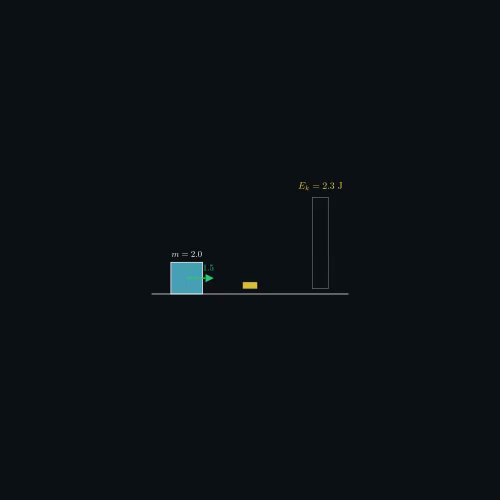
\includegraphics[width=0.82\linewidth, keepaspectratio]{KineticEnergyScene.png}
            
            \vspace{0.1cm}
            {\tiny \textcolor{gray}{\textit{Non-linear scaling: $E_k \propto m$ and $E_k \propto v^2$}}}
        \end{column}

        % Cột phải: Khung Physical Examples
        \begin{column}{0.54\textwidth}
            \begin{block}{Physical Examples}
                \small
                \begin{itemize}
                    \item \textbf{Kinetic energy}:
                    \[
                        E_k = \frac{1}{2}mv^2
                    \]
                    ($m$ is mass, $v$ is velocity).
                    
                    \vspace{0.1cm}
                    \item \textbf{Potential energy}:
                    \[
                        E_p = mgh
                    \]
                    ($m$ is mass, $h$ is height).
                \end{itemize}
            \end{block}
        \end{column}
    \end{columns}
\end{frame}

\end{document}
